\section{Doorway Detection Node} \label{doorway_impl}

The input data for the doorway detection node are the point clouds from the upward looking RGBD-camera and the range measurements from the LIDAR. The most recent range measurements from the LIDAR are stored for further processing. When a new point cloud arrives and the robot has moved considerably since the last execution of the doorway detection, the doorway detection is started. The movement check is done because of performance reasons and to avoid redundant information in the mapping. The output is a set of doorway detections represented as an array of poses in the robot coordinate frame.

The first step is to transform the point cloud from the coordinate frame of the camera into the coordinate frame of the robot using the known static transformation. This transformation was determined manually. First, the z-coordinate, the pitch angle, and the roll angle were determined by comparing the point cloud of the camera with a ceiling of known height. The x-coordinate, y-coordinate, and yaw angle were determined by comparing the point cloud with the laser scan in front of a room corner. In a second step two subsets of points are extracted from the point cloud, one subset containing only points with a height between 1.95\,m and 2.05\,m and one subset containing only points lower than 1.95\,m. Both subsets of points are projected onto the ground and converted into 2D images represented as OpenCV matrices, as shown in Listing \ref{downprojPoints}. The \texttt{resolution} and the \texttt{origin} specify the conversion between the robot coordinates and the image coordinates. The resulting images are shown in Figure \ref{fig:door detection precedure} (a) and (b). From the left image it can be seen that not only points of the upper part of the door frame are at about 2\,m height, but also points on the walls beside the doorway. The purpose of the second image, which also contains those walls, is to eliminate the undesired pixels from the walls. Therefore the second image is subtracted from the first one. Applying the morphological operations closing, to fill possible holes, and opening, to remove stray pixels, results in the filtered image shown in Figure \ref{fig:door detection precedure} (c).

\begin{minipage}{\linewidth}
\begin{lstlisting}[caption=Projection of points into corresponding image,frame=single, label=downprojPoints]
for(point in pointCloud){
  if(point.z>=1.95 and point.z<=2.05)
    at2mImage(point.y*resolution+origin.y,point.x*resolution+origin.x) = 255
  if(point.z<1.95)
    under2mImage(point.y*resolution+origin.y,point.x*resolution+origin.x) = 255
}
\end{lstlisting}
\end{minipage} 

\begin{figure}[h]
\centering
  \subfloat[Projection onto the ground of points at about 2\,m]{{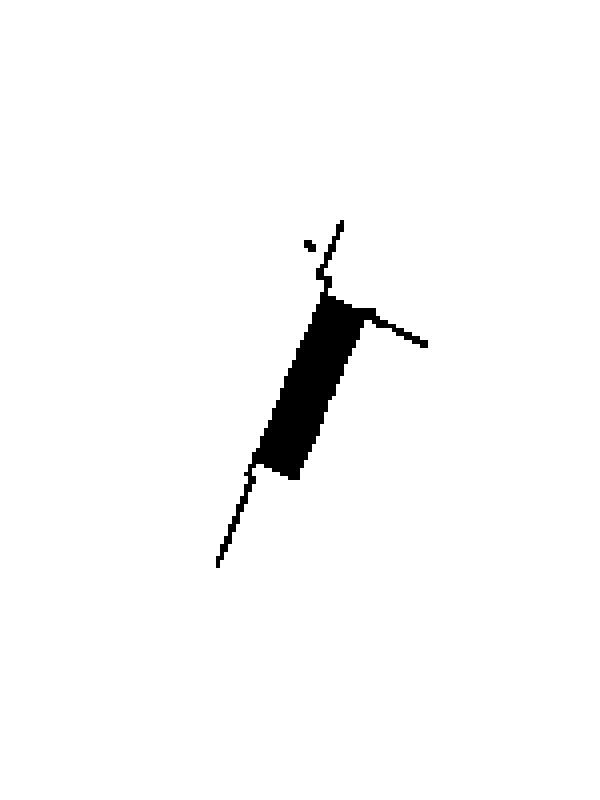
\includegraphics[width=0.3\textwidth, trim = 100 200 150 200, clip]{figures/5occ_orig.png} }}%
  \quad
  \subfloat[Projection onto the ground of points lower than 1.95\,m]{{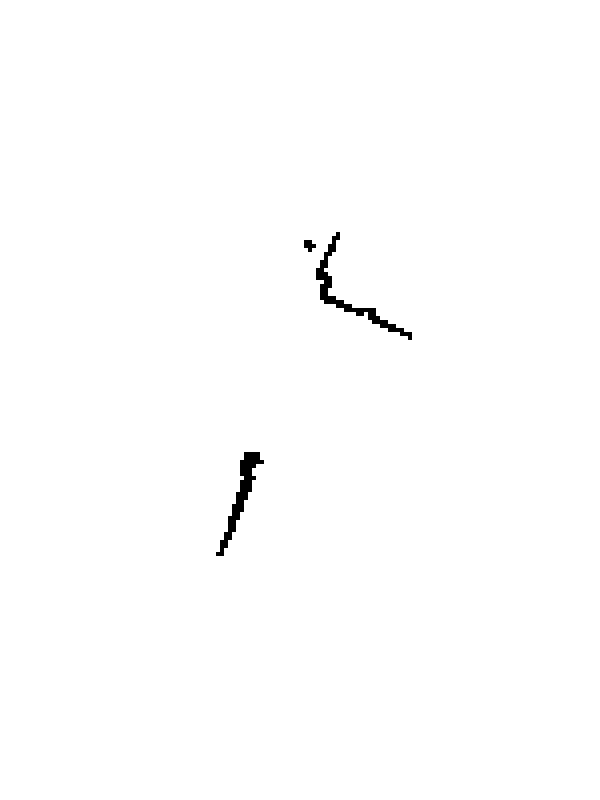
\includegraphics[width=0.3\textwidth, trim = 100 200 150 200, clip]{figures/5occ_under.png} }}%
  \quad
  \subfloat[Filtered image]{{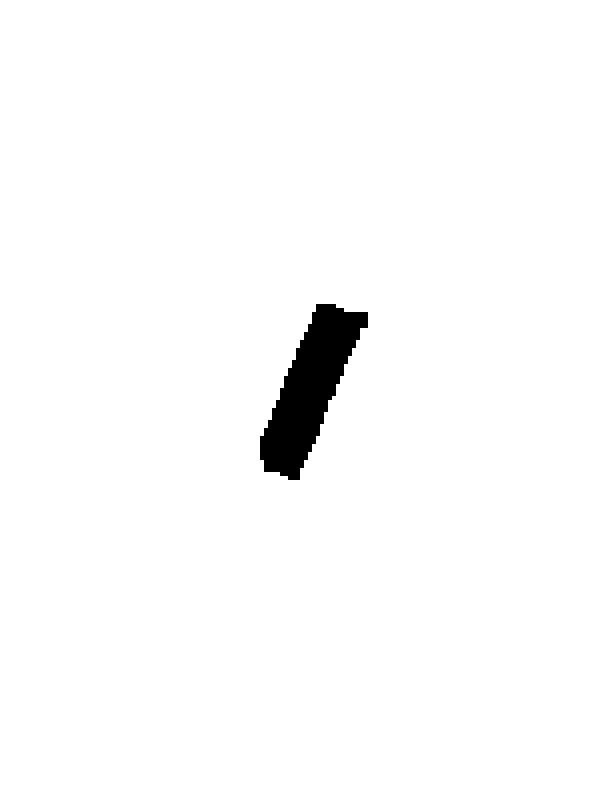
\includegraphics[width=0.3\textwidth, trim = 100 200 150 200, clip]{figures/5occ_filtered.png} }}%
  \caption[Doorway detection procedure]{Preprocessing of the doorway detection}
  \label{fig:door detection precedure}
\end{figure}

The filtered image is searched for contours and around every contour found a minimum area rectangle is fitted. Both is done using OpenCV functions. This is depicted in Figure \ref{door res}, where only one contour was found. All rectangles with $d<0.05\,m \wedge d>0.5\,m \wedge w<0.6\,m$ are ruled out. The width and depth can be converted from pixels to meters using the same resolution as in the conversion into an image.

To execute the other checks described in Section \ref{DoorwayDetection}, the latest laser scan from the LIDAR has to be transformed into the correct coordinate frame. Laser scan and point cloud are usually not acquired at the same time, so robot movement in the time between the measurements has also to be considered. This is done using the tf library, which allows to specify not only the coordinate frames when accessing a transformation but also the time of interest. Three areas are defined in Figure \ref{door res}. For every area the number of points from the transformed laser scan within the area are counted. If the sum of points in the red areas is less than 5 and the number of points in the green area is greater than 30, a doorway is found. The former is necessary for a doorway to be not blocked and the parameter was chosen to be 5 to allow some outliers in the laser scan. The latter is necessary as there have to be walls beside the doorway and the parameter was found in tests. If the rectangle was classified as doorway, the pose of the doorway is estimated as described in Section \ref{DoorwayDetection} and added to the result array. This is done for all fitted rectangles fulfilling the size constrains, so the result is an array containing all detected doorways.
\begin{figure}[h]
  \centering
  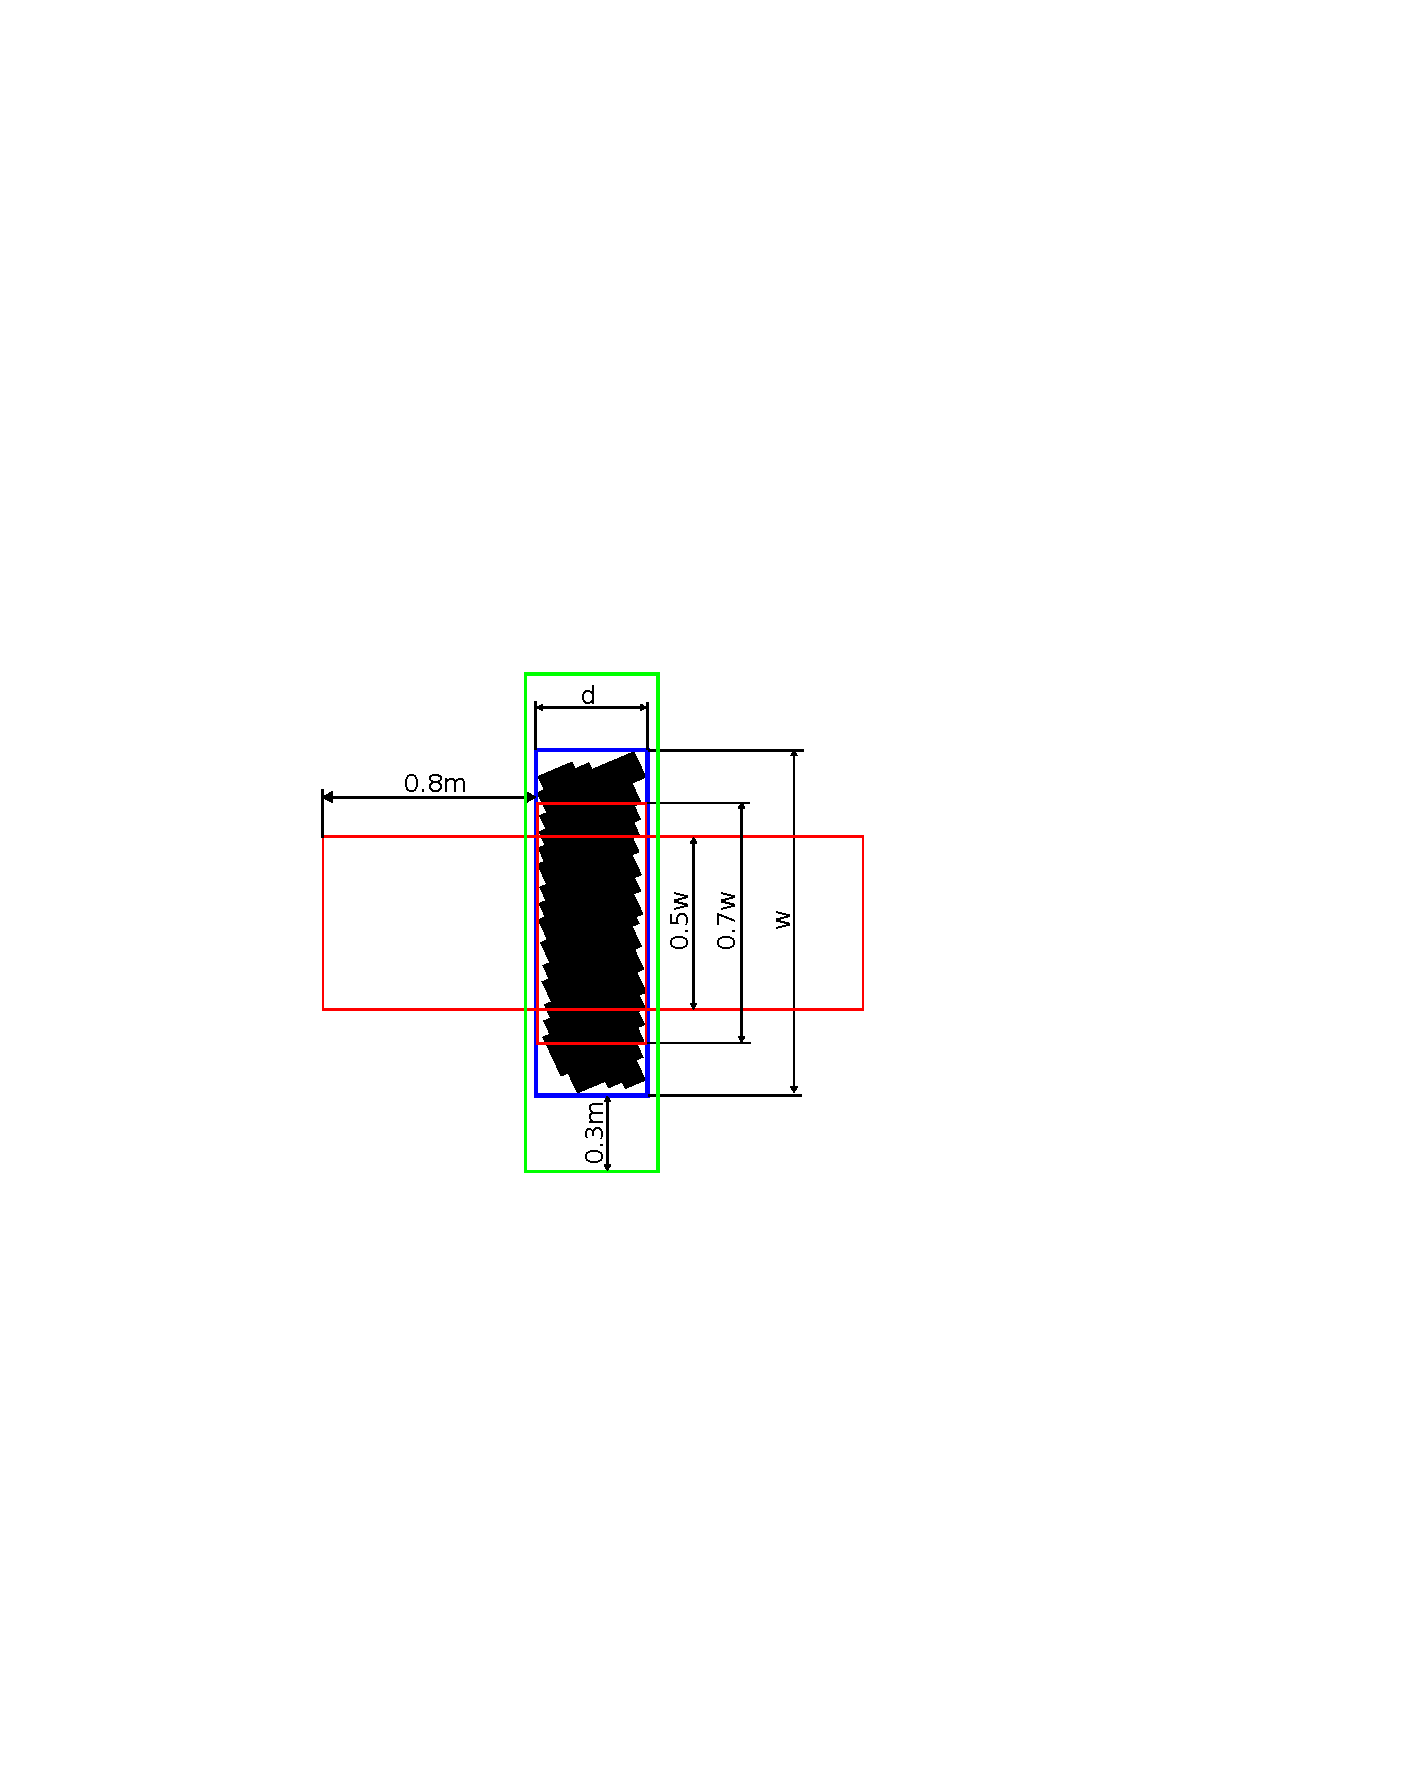
\includegraphics[angle=-24,origin=c,width=0.6\textwidth,trim=100 280 250 320,clip]{figures/5occ_res.pdf} 
  \caption[Door detection area specifications]{The minimum area rectangle (blue) around the filtered doorway contour (black) and specifications of the areas for the doorway check; the number of points from the laser scan has to be less than a threshold in the red rectangles and greater than another threshold in the green rectangle for a doorway being detected}
  \label{door res}
\end{figure}